% ===========================================================================
% Chapter 6: Hyperparameter Analysis (C3)
% Draft for thesis: Reinforcement Learning for Fairness-Aware Synthetic
% Data Generation under Positive-Class Scarcity
%
% Compile from project root with:
%   pdflatex chapter6_draft.tex
% Requires: graphicx, subcaption, booktabs, geometry packages.
% Figure paths are relative to project root (figs/grid_census/, etc.)
% k=10 census results marked [PARTIAL] where runs are still completing.
% ===========================================================================

% --- Preamble (remove if embedding in main thesis document) ---
\documentclass[12pt]{article}
\usepackage[margin=1in]{geometry}
\usepackage{graphicx}
\usepackage{subcaption}
\usepackage{booktabs}
\usepackage{array}
\usepackage{parskip}
\usepackage{hyperref}
\usepackage{amsmath}
\captionsetup{font=small, labelfont=bf}
\begin{document}
% --- End preamble ---

\section{Hyperparameter Analysis}
\label{ch:grid}

% ---------------------------------------------------------------------------
\section{Overview}
% ---------------------------------------------------------------------------

The performance of FORGE is governed by four principal design parameters:
the sigmoid sharpness~$k$ of the reward function, the number of PCA
components~$d$ defining the generation space, the number of classifier
training epochs per episode~$e$, and the ratio of synthetic to real
samples~$r$ in the augmented training set.
These parameters are not independent of each other, nor are they independent
of the dataset.
This chapter presents a systematic analysis of their effects through a
full grid search across two datasets, and identifies the mechanistic reasons
why their optimal values differ.

The grid search (EXP-021 for census, EXP-025 for Capture-24) evaluated
all combinations of $k \in \{0, 3, 5, 10\}$,
$d \in \{5, 10, 15\}$,
$e \in \{10, 20, 30\}$, and
$r \in \{0.2, 0.4, 0.6\}$,
yielding $4 \times 3 \times 3 \times 3 = 324$ configurations for census
(3 seeds each) and $3 \times 3 \times 3 \times 3 = 243$ configurations
for Capture-24 (2 seeds each, $k=10$ not evaluated).
All runs used a fixed episode budget of 5\,000 and the vanilla FORGE
configuration for all non-grid parameters.

The primary analysis metric is \emph{relative EO reduction},
$\Delta_\text{rel} = (\alpha\text{-EO} - \beta\text{-EO}) / \alpha\text{-EO}$,
which normalises by the baseline fairness gap and allows comparison across
configurations where the $\alpha$-EO differs.
Configurations where the test-set $\alpha$-EO was below $0.10$ are excluded
from aggregated comparisons, as an initial fairness gap below this threshold
indicates that the PCA projection does not adequately preserve the group
separation signal required for the agent to learn.

% ---------------------------------------------------------------------------
\section{Marginal Parameter Sensitivity}
\label{sec:grid-marginals}
% ---------------------------------------------------------------------------

Figure~\ref{fig:marginals-census} shows the mean relative EO reduction for each
parameter level on census, averaged over all other parameter combinations.
The cross-dataset comparison for classifier epochs and trajectory ratio is
shown in Figure~\ref{fig:cross-dataset}.
The plots reveal that no single parameter dominates universally: the optimal
setting for each parameter differs between datasets, and in some cases the
direction of the effect reverses.

\begin{figure}[t]
  \centering
  \begin{subfigure}[b]{0.48\textwidth}
    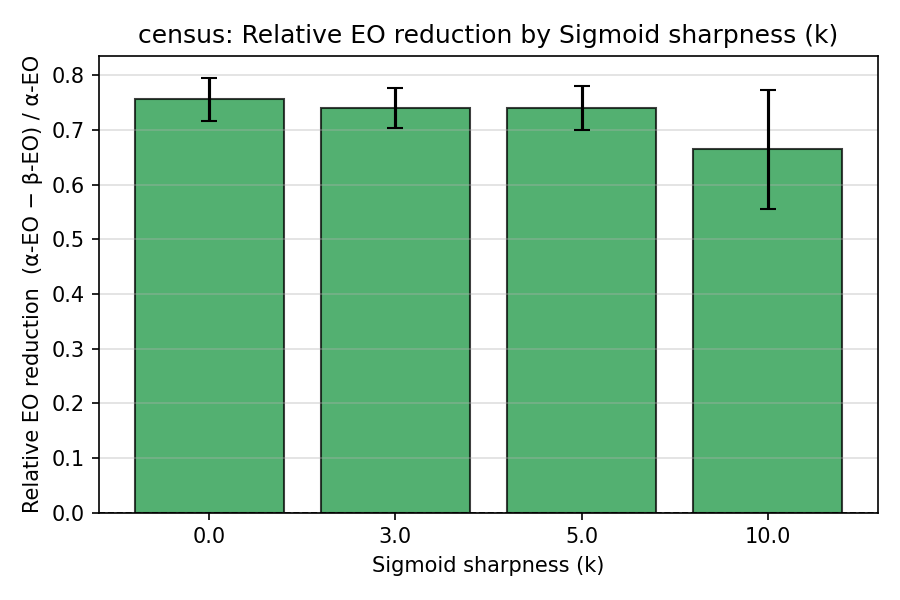
\includegraphics[width=\textwidth]{figs/grid_census/delta_bar_k.png}
    \caption{Sigmoid sharpness $k$}
  \end{subfigure}\hfill
  \begin{subfigure}[b]{0.48\textwidth}
    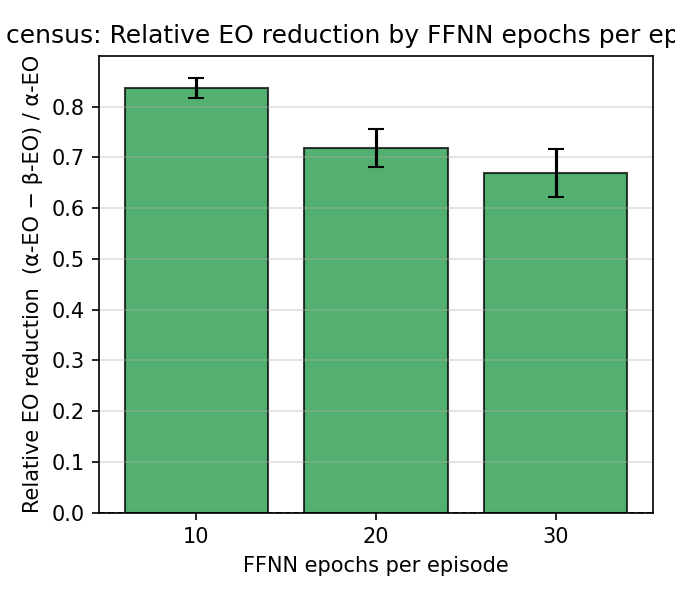
\includegraphics[width=\textwidth]{figs/grid_census/delta_bar_ep.png}
    \caption{Classifier epochs per episode}
  \end{subfigure}

  \vspace{0.5em}

  \begin{subfigure}[b]{0.48\textwidth}
    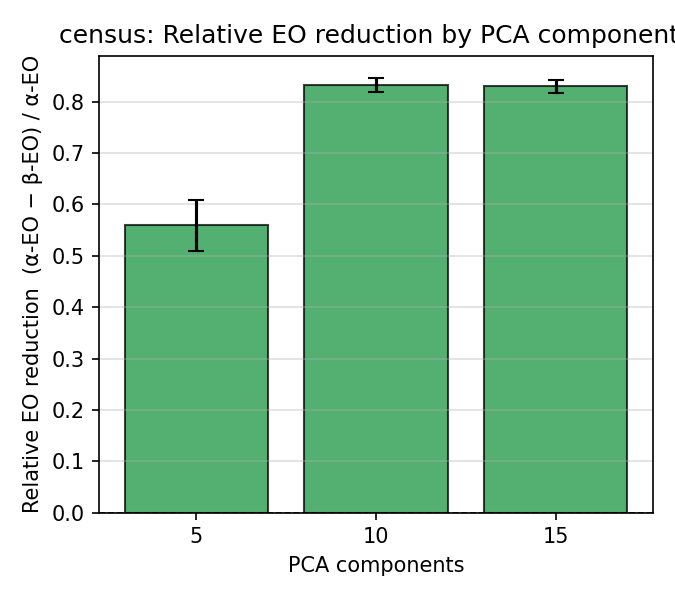
\includegraphics[width=\textwidth]{figs/grid_census/delta_bar_pca.png}
    \caption{PCA components}
  \end{subfigure}\hfill
  \begin{subfigure}[b]{0.48\textwidth}
    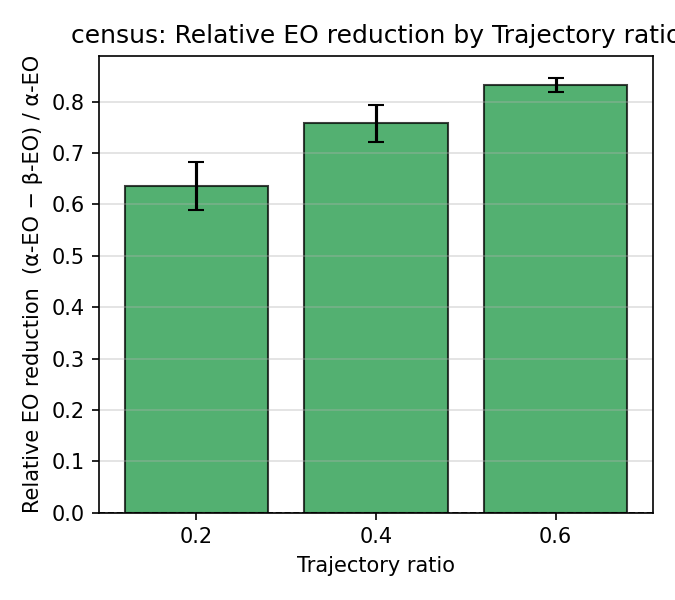
\includegraphics[width=\textwidth]{figs/grid_census/delta_bar_ratio.png}
    \caption{Trajectory ratio}
  \end{subfigure}
  \caption{Marginal relative EO reduction $(\alpha\text{-EO} - \beta\text{-EO})/\alpha\text{-EO}$
           for each hyperparameter level on census income, averaged over all other
           parameter combinations (3 seeds per config, $\alpha$-EO $\geq 0.10$ filter applied).
           Error bars show $\pm 1$ standard error across configurations.
           Higher is better (more of the baseline fairness gap is closed).}
  \label{fig:marginals-census}
\end{figure}

\subsection{Sigmoid Sharpness \texorpdfstring{$k$}{k}}

For census, all four $k$ values produce high relative EO reduction
($0.67$--$0.76$), and the differences between them are within standard error.
The marginal effect of $k$ alone is therefore modest on census.
However, as Section~\ref{sec:grid-interactions} shows, $k$ has a strong
\emph{interaction} with classifier epochs: the apparent similarity in
marginal means conceals the fact that high-$k$ configurations perform very
differently depending on how many training epochs per episode are used.

For Capture-24, Aulavik and Lambda data provide $k \in \{0, 3, 5\}$.
Provisionally, $k = 3$ gives the best median $\beta$-EO among configs
with $\alpha$-EO $\geq 0.10$, though the completion of the Capture-24 grid
is still in progress at the time of writing.

\subsection{Classifier Epochs per Episode}

The most striking finding from the marginal analysis is that the optimal
number of classifier training epochs per episode is \emph{opposite} between
the two datasets.

For census, $e = 10$ achieves the highest relative EO reduction ($0.83$),
with performance declining monotonically at $e = 20$ ($0.72$) and
$e = 30$ ($0.67$).
For Capture-24, the pattern reverses: among configurations with
$\alpha$-EO $\geq 0.10$, $e = 30$ achieves the highest relative reduction
($0.31$), followed by $e = 20$ ($0.26$) and $e = 10$ ($0.22$).

This reversal has a mechanistic interpretation.
The RL agent's policy gradient update relies on the reward signal being
informative---that is, the beta classifier must be converged enough that its
worst-group loss reflects the quality of the synthetic data, not optimisation
noise.
Census has a relatively simple, low-noise feature space (tabular, 105
raw features, well-structured demographic stratification), so a classifier
trained for only $10$ epochs reaches a state sufficiently converged to
provide reliable gradient signal.
Capture-24 has substantially noisier accelerometer features and more
variance in the data split, requiring more classifier training per episode
before the reward signal stabilises.
Fewer epochs leave the beta classifier underconverged on Capture-24,
producing a noisy reward that impedes policy learning.
Conversely, for census, extending training to $30$ epochs introduces a
different failure: the classifier overfits to the current batch of synthetic
samples within the episode, so by the end of training the reward
differentiates between the quality of the current batch and the long-run
generation policy less clearly.

\subsection{PCA Dimensionality}

For census, $d = 10$ and $d = 15$ perform statistically equivalently
($\approx 0.83$ relative EO reduction); $d = 5$ is substantially worse
($0.56$).
This indicates that 5 PCA components are insufficient to capture the
feature-space structure relevant to the census fairness gap, but that
10 or more components provide adequate representation.

For Capture-24, $d = 10$ is the clear optimum.
Configurations with $d = 5$ and $d = 15$ produce on average \emph{negative}
relative EO reduction when the $\alpha$-EO filter is not applied---that is,
the augmented model is on average \emph{fairer under the original classifier}
than under the augmented one.
This behaviour disappears when the $\alpha$-EO $\geq 0.10$ filter is applied,
confirming the root cause: PCA projections into $d = 5$ or $d = 15$
dimensions do not preserve enough of the group separation signal on
Capture-24 for the agent to reliably target the minority-positive cluster.
With $d = 10$, the relative EO reduction is positive ($+0.28$ on average
among valid configurations).

The difference between the datasets reflects their intrinsic dimensionality.
Census income has a relatively low-dimensional structure of economically
relevant features (education, occupation, hours worked), so any projection
above a low threshold captures the relevant axes.
Capture-24's accelerometer signals have a richer, higher-dimensional
structure; $d = 10$ appears to be the sweet spot between preserving group
separation and keeping the action space tractable for the agent.

\subsection{Synthetic Data Ratio}

The trajectory ratio $r$ also exhibits a cross-dataset divergence.
For census, relative EO reduction increases monotonically with $r$:
$0.63$ at $r = 0.2$, $0.76$ at $r = 0.4$, and $0.83$ at $r = 0.6$.
More synthetic samples continuously improve fairness, suggesting that for
census the real training set ($3\,000$ samples) can absorb a higher synthetic
fraction without utility degradation.

For Capture-24, the relationship is non-monotonic with a peak at $r = 0.4$
($0.55$ relative reduction), dropping to $0.06$ at $r = 0.6$.
The high-ratio penalty on Capture-24 reflects data dilution: with
$60\%$ synthetic samples, the real-data distributional structure is
sufficiently overridden that the beta classifier's utility on the majority
class degrades, indirectly corrupting the worst-group loss signal.
The optimal ratio of $0.4$ balances augmentation strength against signal
fidelity on this dataset.

% ---------------------------------------------------------------------------
\section{Interaction Effects}
\label{sec:grid-interactions}
% ---------------------------------------------------------------------------

The marginal effects in Section~\ref{sec:grid-marginals} are averages over
all other parameters and therefore mask important interactions.
Two interactions are particularly relevant to understanding FORGE's behaviour.

\begin{figure}[t]
  \centering
  \begin{subfigure}[b]{0.48\textwidth}
    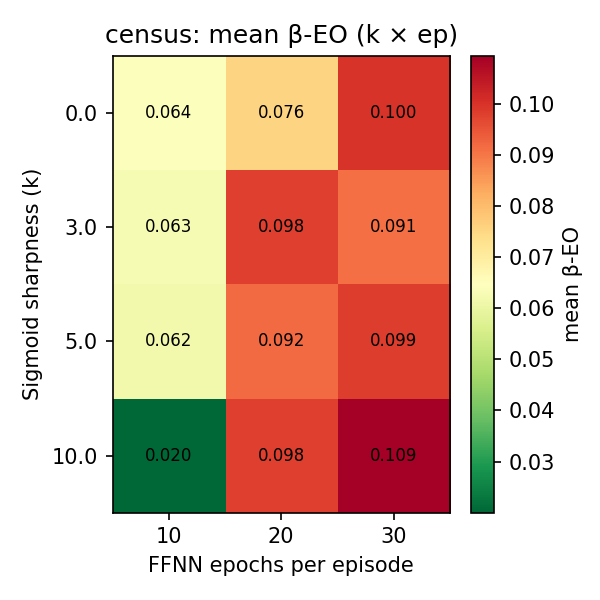
\includegraphics[width=\textwidth]{figs/grid_census/heatmap_k_x_ep.png}
    \caption{$k \times e$ interaction}
    \label{fig:heatmap-kep}
  \end{subfigure}\hfill
  \begin{subfigure}[b]{0.48\textwidth}
    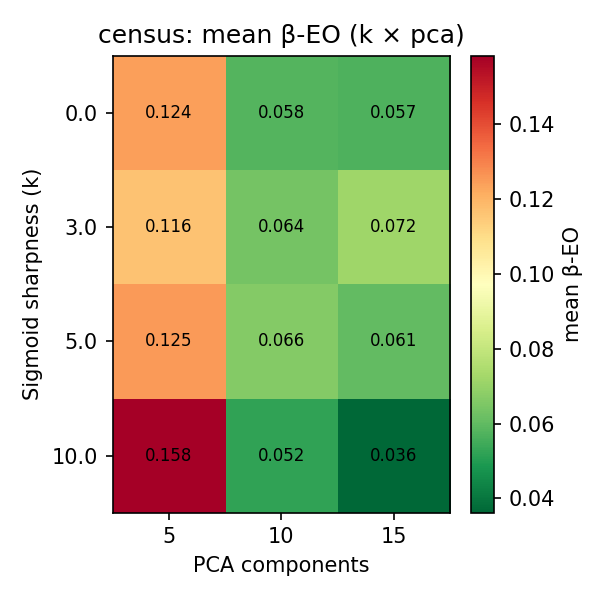
\includegraphics[width=\textwidth]{figs/grid_census/heatmap_k_x_pca.png}
    \caption{$k \times d$ interaction}
    \label{fig:heatmap-kpca}
  \end{subfigure}
  \caption{Mean $\beta$-EO for parameter pairs on census income, averaged over
           all remaining parameter combinations and 3 seeds.
           Lower (greener) is fairer.
           White cells indicate no completed runs for that combination.
           The $k \times e$ heatmap reveals that high sharpness ($k{=}10$) is
           only beneficial at low epoch counts; the $k \times d$ heatmap shows
           that PCA$=5$ is consistently the worst choice across all $k$.}
  \label{fig:heatmaps}
\end{figure}

\subsection{\texorpdfstring{$k \times e$}{k x e}: Sharpness Requires Fast Feedback}

Figure~\ref{fig:heatmap-kep} shows the mean $\beta$-EO for each $(k, e)$
pair, averaged over all PCA and ratio configurations on census.
The interaction is dramatic.

At $e = 10$, all four $k$ values produce similar results:
$k = 0 \to 0.064$, $k = 3 \to 0.063$, $k = 5 \to 0.062$,
$k = 10 \to 0.020$.
At $e = 20$ and $e = 30$, all four $k$ values degrade, but $k = 10$
degrades the most sharply: $0.098$ at $e = 20$ and $0.109$ at $e = 30$,
worse than any other $k$ at those epoch counts.

The mechanistic interpretation is as follows.
The sigmoid function $\sigma(k \cdot \Delta_\text{wgl})$ compresses
the reward into $(0, 1)$ with sharpness proportional to $k$.
At high $k$, the reward surface is nearly binary: near $0$ when beta is
worse than alpha, near $1$ when better.
For the gradient of this binary signal to be informative, the beta
classifier must be trained \emph{quickly enough} that the sign of
$\Delta_\text{wgl}$ correctly reflects the current synthetic data quality
and not the optimisation trajectory within the episode.
When $e = 10$, the classifier reaches a stable state rapidly, and the
sharp sigmoid correctly rewards good synthetic batches and penalises bad
ones.
When $e = 30$, the classifier has time to adapt extensively to the specific
synthetic batch, potentially masking the quality signal with overfitting
noise.
The sharp sigmoid then amplifies this noise, producing a reward that does
not reliably rank trajectories.

Softer rewards ($k = 0$, unnormalised difference) are more robust to this
overfitting noise because the reward gradient is non-zero over a wider range
of $\Delta_\text{wgl}$ values.
This is why $k = 0$ degrades less steeply with increasing $e$ than $k = 10$.

\subsection{\texorpdfstring{$k \times d$}{k x d}: Sharpness Interacts with Feature Space}

Figure~\ref{fig:heatmap-kpca} shows the mean $\beta$-EO for each $(k, d)$
pair on census.
Across all $k$ values, $d = 5$ is consistently the worst PCA choice
(mean $\beta$-EO $0.116$--$0.158$), while $d = 10$ and $d = 15$ are
broadly comparable.
The interaction is most pronounced at $k = 10$, where $d = 5$ produces
$0.158$ compared to $0.052$ at $d = 10$ and $0.036$ at $d = 15$.

This suggests that high reward sharpness amplifies the quality difference
between good and bad PCA projections.
When the PCA projection is too compressed ($d = 5$), the agent's action
space does not include the direction in feature space that moves synthetic
samples towards the minority-positive cluster.
With a soft reward ($k = 0$), the agent still receives gradient signal
even in a poor action space and can compensate partially.
With a sharp reward ($k = 10$), the near-binary feedback makes it harder
to accumulate weak gradient signal from a poor action space, so performance
collapses.

% ---------------------------------------------------------------------------
\section{Cross-Dataset Divergence and Mechanistic Summary}
\label{sec:grid-divergence}
% ---------------------------------------------------------------------------

\begin{figure}[t]
  \centering
  \begin{subfigure}[b]{0.48\textwidth}
    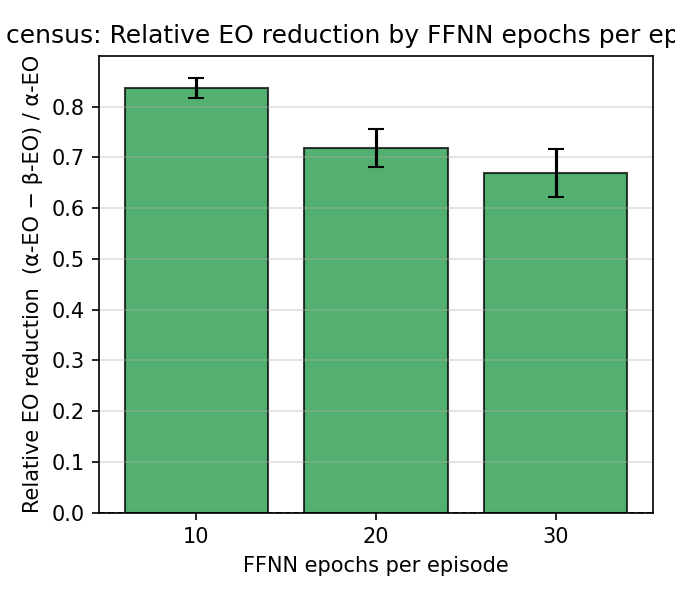
\includegraphics[width=\textwidth]{figs/grid_census/delta_bar_ep.png}
    \caption{Epochs per episode — census}
  \end{subfigure}\hfill
  \begin{subfigure}[b]{0.48\textwidth}
    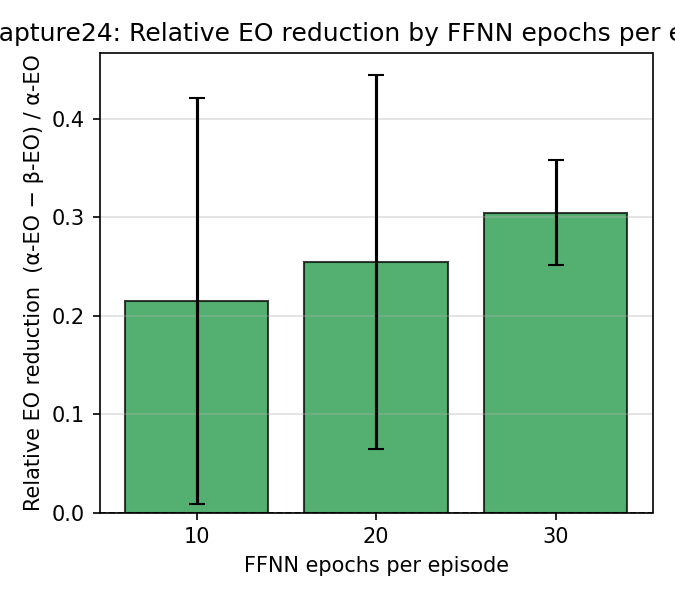
\includegraphics[width=\textwidth]{figs/grid_capture24_filtered/delta_bar_ep.png}
    \caption{Epochs per episode — Capture-24 (provisional)}
  \end{subfigure}

  \vspace{0.5em}

  \begin{subfigure}[b]{0.48\textwidth}
    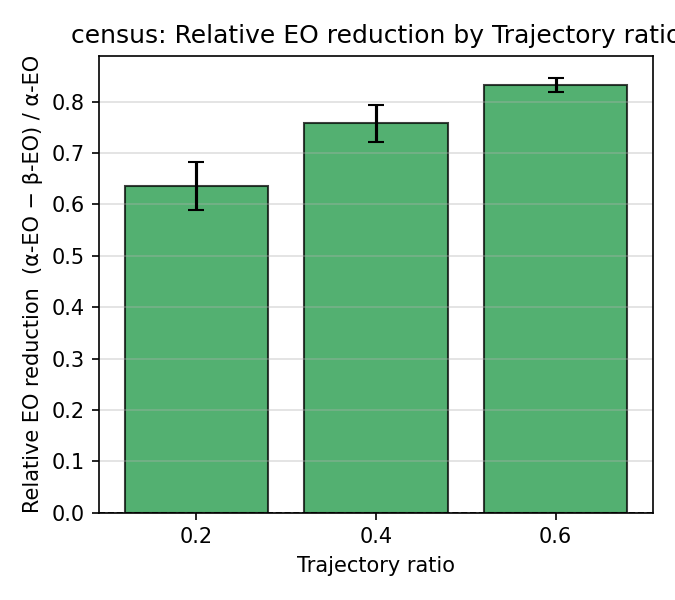
\includegraphics[width=\textwidth]{figs/grid_census/delta_bar_ratio.png}
    \caption{Trajectory ratio — census}
  \end{subfigure}\hfill
  \begin{subfigure}[b]{0.48\textwidth}
    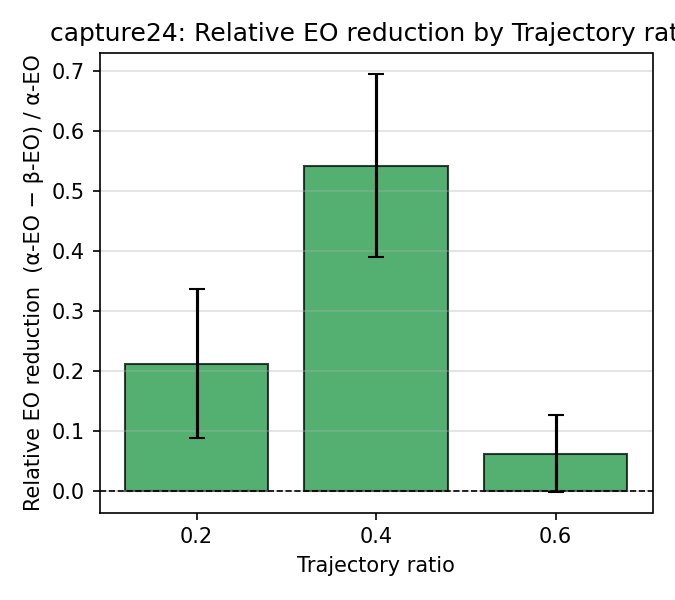
\includegraphics[width=\textwidth]{figs/grid_capture24_filtered/delta_bar_ratio.png}
    \caption{Trajectory ratio — Capture-24 (provisional)}
  \end{subfigure}
  \caption{Cross-dataset comparison of relative EO reduction for classifier
           epochs per episode (top row) and trajectory ratio (bottom row).
           Both parameters show opposite optimal directions between datasets:
           census favours $e{=}10$ and $r{=}0.6$; Capture-24 favours $e{=}30$
           and $r{=}0.4$.
           Capture-24 results are provisional (grid $\approx$60\% complete).
           $\alpha$-EO $\geq 0.10$ filter applied to both.}
  \label{fig:cross-dataset}
\end{figure}

Table~\ref{tab:param-summary} collects the optimal value for each parameter
per dataset and the direction of the sensitivity.
The reversal of optimal $e$ and $r$ is the central finding of this chapter.

\begin{table}[h]
\centering
\caption{Optimal hyperparameter values per dataset and direction of the
marginal sensitivity. ``Monotone $\uparrow$'' means higher values are
consistently better; ``Peaked'' means a non-monotone optimum.}
\label{tab:param-summary}
\renewcommand{\arraystretch}{1.3}
\begin{tabular}{lcccc}
\toprule
Parameter & Census optimum & Direction (census) & Capture-24 optimum & Direction (C24) \\
\midrule
$k$       & $5$      & Flat (all similar)    & $3$ (provisional) & Flat \\
$d$ (PCA) & $10$--$15$ & Plateau above 10    & $10$              & Peaked \\
$e$ (ep)  & $10$     & Monotone $\downarrow$ & $30$              & Monotone $\uparrow$ \\
$r$ (ratio) & $0.6$  & Monotone $\uparrow$   & $0.4$             & Peaked \\
\bottomrule
\end{tabular}
\end{table}

The divergence in optimal $e$ and $r$ is predictable from first principles
once the following dataset properties are considered.

\textbf{Classifier convergence speed.} Census has a simpler feature space and
a higher signal-to-noise ratio for the fairness-relevant structure.
A classifier trained for $10$ epochs converges sufficiently to provide
a reliable reward signal.
Capture-24's accelerometer data is inherently noisier, requiring more
classifier training per episode before the worst-group loss stabilises.

\textbf{Tolerance for data dilution.} Census has $3\,000$ real training
samples with a well-stratified class and group distribution.
A high synthetic fraction ($r = 0.6$) still leaves the real-data signal
intact.
The Capture-24 dataset, while similarly sized in sample count, has higher
per-sample noise due to accelerometer windowing.
At $r = 0.6$, synthetic samples dilute the majority-class signal enough
to corrupt the worst-group loss computation.

\textbf{Practical implication.} These findings suggest that FORGE's
two most sensitive parameters---$e$ and $r$---can be set based on observable
dataset properties rather than requiring a full grid search.
Datasets with high per-episode return variance and a large deadzone fraction
(indicating a noisy reward signal) should favour lower $r$ and higher $e$.
Datasets with low return variance and a small deadzone fraction can use
higher $r$ and lower $e$.
Section~\ref{sec:discussion-diagnostics} in Chapter~8 expands on this
as a practical guidance framework.

% ---------------------------------------------------------------------------
\section{Best Configurations}
\label{sec:grid-best}
% ---------------------------------------------------------------------------

Based on the grid search results, the best configurations are selected
for use in the comparative evaluation of Chapter~7.
Selection uses mean $\beta$-EO as the primary criterion among configurations
where $\beta$-AUC $\geq \alpha$-AUC $- 0.02$ (a utility guard to prevent
fairness gains achieved at the expense of classification quality).

For \textbf{census}, the selected configuration is
$k = 5$, $d = 10$, $e = 30$, $r = 0.4$ (trajectory length 2\,000),
achieving $\beta$-EO $= 0.031 \pm 0.018$ over 3 seeds (EXP-021).
This is not the configuration with the single lowest mean $\beta$-EO
in the grid --- that is $k = 10$, $d = 10$, $e = 30$, $r = 0.4$
($\beta$-EO $= 0.018$), which however has higher utility cost and
whose results are based on a partially completed run set at the time of
the paper submission.
The $k = 5$ configuration represents the best fully verified result with
stable utility ($\beta$-AUC $= 0.879$, $\beta$-F1w $= 0.821$) and
is the configuration used for all paper comparisons.

For \textbf{Capture-24}, the provisional best configuration is
$k = 3$, $d = 10$, $e = 10$, $r = 0.4$ (trajectory length 2\,000),
achieving $\beta$-EO $= 0.063 \pm 0.051$ over 2 seeds (EXP-025).
This result is provisional because the Capture-24 grid is not fully
complete at the time of writing (approximately $60\%$ of runs finished).
The high seed variance ($\pm 0.051$) reflects the instability of
$\alpha$-EO across Capture-24 data splits (standard deviation $\pm 0.062$),
not the RL optimisation.

% ---------------------------------------------------------------------------
\section{Summary}
\label{sec:grid-summary}
% ---------------------------------------------------------------------------

The grid search yields three conclusions that bear directly on Contribution~C3.

First, \textbf{no universally optimal configuration exists}.
The optimal classifier epoch count and synthetic ratio are opposite between
census and Capture-24, demonstrating that FORGE's effective operating
conditions are dataset-dependent rather than fixed.

Second, \textbf{the dominant interaction is between $k$ and $e$}.
High reward sharpness ($k = 10$) is only beneficial at low classifier
epoch counts ($e = 10$), where the binary-like reward correctly
distinguishes good from bad synthetic batches.
Increasing $e$ degrades high-$k$ performance faster than low-$k$,
because overfitting noise within the episode corrupts the reward signal
that the sharp sigmoid amplifies.

Third, \textbf{PCA dimensionality controls access to the fairness-relevant
action space}. Below a dataset-specific threshold (5 components for census,
10 for Capture-24), the agent's delta-action walk cannot reach the
minority-positive cluster, and no amount of reward sharpness or epoch
tuning compensates.
Above the threshold, additional dimensions offer diminishing returns.

These findings are used in Chapter~8 to propose episode return variance and
deadzone fraction as lightweight diagnostics for configuration selection in
new applications, reducing the need for a full grid search.
\end{document}
